\documentclass[runningheads]{llncs}

% General LaTeX macros
\usepackage{xcolor}
\usepackage{multirow}
\usepackage{bigdelim}
\usepackage{makecell}
\usepackage{booktabs}
\usepackage{textcomp}
\usepackage{emptypage}
\usepackage[T1]{fontenc}
\usepackage[utf8]{inputenc}

\usepackage{algorithm}
\usepackage{algpseudocode}
\raggedbottom

% Math === === === === === === === === === ===
\usepackage{leftindex}
\usepackage{mathtools}
\usepackage{siunitx}
\usepackage{enumitem}
\usepackage{amsmath, amssymb}
\DeclareMathOperator*{\argmax}{argmax}
\newcommand{\nvec}[1]{\underline{#1}}

\usepackage{overpic}
\graphicspath{ {./figures/} }

\usepackage{hyperref}
\renewcommand\UrlFont{\color{blue}\rmfamily}

% ML === === === === === === === === === ======
\newcommand{\dataset}{\boldsymbol{\mathit{X}}}
\newcommand{\labels}{\nvec{y}}
\newcommand{\sample}{\nvec{x}}
\newcommand{\feature}{\mathtt{f}}
\newcommand{\fvector}{\nvec{\mathtt{f}}}
\newcommand{\fset}{\mathcal{F}}
\newcommand{\fsubset}{\bar{\mathcal{F}}}
\newcommand{\pmset}{\mathcal{G}}

% RL === === === === === === === === === ======
\newcommand{\policy}{\boldsymbol{\pi}}
\newcommand{\optpolicy}{\boldsymbol{{\pi}^*}}
\newcommand{\vicon}{Vicon\textsuperscript{\textregistered{}}}
\newcommand{\mbbody}{MobileBody\textsuperscript{\textregistered{}}}

\begin{document}
%
\title{Interdisciplinary Poststroke Gait Assessment with Patient-Specific Feature and Model Selection via Deep Q-Learning}
\titlerunning{Gait Assessment with Patient-Specific Feature \& Model Selection via DQL}

\author{
  Jin Cheng Liaw \inst{1}\orcidID{0009-0006-0719-0363} \and
  Chang Zheng Chiang \inst{1*} \and
  Dominik Raab \inst{1}\orcidID{0000-0003-4514-1053} \and
  Mario Siebler \inst{2,3} \and
  Harald Hefter \inst{3} \and
  Dörte Zietz \inst{4} \and
  Marcus Jäger \inst{5,6} \and
  Andrés Kecskeméthy \inst{1} \and
  Francisco Geu Flores \inst{1}\orcidID{0000-0002-8106-0894}
}
%
\authorrunning{J.C. Liaw et al.}

\institute{
  Chair of Mechanics and Robotics, University of Duisburg-Essen, Lotharstr. 1, 47057 Duisburg, Germany\\
  \email{\{jin.liaw, dominik.raab, andres.kecskemethy, francisco.geu\}@uni-due.de}\\
  *\email{czchiang1616@gmail.com} \and
  Mediclin Rehabilitationsforschung gGmbH, Okenstr. 27, 77652 Offenburg, Germany\\
  \email{mario.siebler@mediclin.de} \and
  Department of Neurology, University Hospital Düsseldorf, Moorenstr. 5, 40225 Düsseldorf, Germany\\
  \email{harald.hefter@online.de} \and
  Department of Applied Health Sciences - Physiotherapy, University of Applied Sciences Bochum, Gesundheitscampus 6-8, 44801 Bochum, Germany\\
  \email{doerte.zietz@hs-gesundheit.de} \and
  Department of Orthopedics, Trauma and Reconstructive Surgery, St. Marien-Hospital Mülheim an der Ruhr, Kaiserstr. 50, 45468 Mülheim an der Ruhr, Germany\\
  \email{m.jaeger@contilia.de} \and
  Chair of Orthopedics and Trauma Surgery, University of Duisburg-Essen, Hufelandstr. 55, 45147 Essen, Germany
}

\maketitle

\begin{abstract}
  Designing personalized therapy for poststroke gait rehabilitation often involves the effort of an interdisciplinary medical team and tedious assessments. An automated gait assessment tool based on gait measurements and interdisciplinary knowledge could help experts with faster gait assessments, while providing objective feedback. The high dimensionality of gait data however, makes it challenging for subsequent analyses. Inspired by the application of Deep Q-Learning in solving multi-step procedures, this study presents a method for dynamic feature and model selection. The search space is formulated as a partially observable Markov Decision Process, where the agent iteratively explores the 680 extracted gait features and various prediction models, to learn optimal patient-specific combinations of feature subsets and prediction models. The model was developed using a dataset of 904 stride pairs from 100 hemiparetic stroke patients. Each patient was evaluated by an interdisciplinary medical board using the Stroke Mobility Score, a multiple-cue clinical observational score comprised of six functional subscores. The agent was trained to approximate optimal decision-making, receiving rewards for accurate predictions and efficient feature selection. Results demonstrated excellent predictive performance, achieving a coefficient of determination ($R^2$) of 0.83 on a held-out test dataset. More importantly, the tool identifies patient-specific key features, that could help highlight specific therapeutic targets for designing personalized poststroke therapy.

%% ORIGINAL
% Designing personalized therapy for poststroke gait rehabilitation often involves the effort of an interdisciplinary medical team and tedious assessments. An automated gait-assessment tool based on gait measurements and interdisciplinary knowledge could help experts with faster gait assessments, while providing objective feedback. However, developing such a tool based on gait data can be challenging due to the high dimensionality of the training datasets typically derived from gait measurements.
%
% While a common approach involves carrying out feature selection on a fixed feature set, this work presents a dynamic feature and model selection approach using reinforcement learning. Hereby, the task of selecting the optimal feature set and corresponding prediction model to map gait data to expert gait-assessment is formulated as a partially observable Markov Decision Process (POMDP), where an agent learns by autonomously exploring different options for each available sample iteratively.
%
% This approach adds a patient-specific component to the gait assessment tool, which could assist clinicians in tailoring personalized therapy.
%
% To achieve this, a dataset is first obtained from 100 hemiparetic stroke-patients which received a clinical examination and a full-body instrumented gait-analysis. An interdisciplinary board of medical experts assigned each patient a Stroke Mobility Score, a multiple-cue clinical observational score comprised of six sub-scores, each pertaining to a functional criterion of gait.
%
% From the measurements, 904 measured stride pairs of 100 patients were obtained, 690 gait features extracted, and the dataset split 70/30 for training and testing. As a preprocessing step, expert knowledge was used to trim the features accordingly, followed by filtering out statistically non-discriminatory features. Within the setting of a POMDP, the agent is allowed to either query a feature or a prediction model, or make a prediction based on the selected feature set and prediction model.
%
% The agent is then rewarded accordingly for each action, before transitioning onto a next state where the process is repeated iteratively. Over the course of many iterations, the agent eventually learns to select an optimal set of actions, given a set of features of a stride pair measurement.
%
% The agent is trained using a Deep Q-Learning algorithm that approximates the Bellman equation by training a deep neural network iteratively on a batch of randomly chosen transitions. The trained agent tested on the test dataset yielded excellent predictive performance, showing a coefficient of determination of 0.85, while delivering patient-specific key features. The delivered patient-specific key features could help clinicians focus on key therapeutic targets, specifically tailored to a patient's needs.

  \keywords{Poststroke gait rehabiliation \and Gait assessment \and Dynamic feature and model selection \and Reinforcement learning \and Deep Q-Learning}
\end{abstract}
% section, subsection, subsubsection, paragraph
\section{Introduction}
Poststroke gait rehabilitation requires a personalized therapy, usually designed by an interdisciplinary medical team via time-consuming assessments \cite{raab2020,liaw2025}. An automated gait assessment tool based on gait measurements and interdisciplinary knowledge could allow for faster poststroke evaluation, while providing relevant feedback via objective analysis of a patient’s status. One major challenge of using gait data for this purpose is its high dimensionality, which is usually met by carrying out feature selection on a fixed feature set. Owing to the individual uniqueness of each patient in terms of physical and functional statuses \cite{lee2020}, we present a dynamic feature and model selection approach using reinforcement learning (RL).

\cite{lee2020} has for instance shown that when performing the ``Bring a Hand to Mouth''-exercise during stroke rehabilitation, different stroke patients compensate for the affected motion in different ways. Beyond inter-patient variability, the relevant biomarkers have also been shown to evolve alongside disease severity. \cite{pistacchi2017} showed for instance how reduced step lengths appeared to be a specific feature of Parkinson's disease in its early stages. As the disease progresses to its moderate stage, gait asymmetry, double-limb support, and increased cadence becomes more characteristic, followed by freezing of gait and reduced balance in its advanced stages. Notably, research \cite{huang2016,biase2020} have highlighted the necessity of adapting the analyzed gait parameters to evolve in tandem with the disease's condition.

In this work, we apply the Deep $Q$-Learning (DQL) algorithm by \cite{mnih2015} to select an optimal set of salient gait features, coupled along with a corresponding prediction model to automatically assess gait poststroke, based on the interdisciplinary knowledge of a medical board. This dynamic approach allows for selecting patient-specific key features, which should be more beneficial over classically selecting a fixed subset of informative features \cite{lee2020,lee2021}. It is after all the therapist's goal to design a \emph{personalized} therapy plan. Moreover, simply presenting a multitude of variables can easily overwhelm a therapist and hinder one from obtaining useful insights \cite{lee2021}. This could in turn aid a clinician in saving precious time \cite{lee2021}, especially in light of the current shortage of medical staff \cite{healthcareburden}. 

\section{Methods}
\subsection{Reinforcement Learning}
RL is a branch of machine learning that deals with learning control laws and policies to interact with an environment, via trial-and-error to achieve a long-term objective \cite{mnih2015,sutton2018,brunton2022}. The learning is guided via feedback, or \emph{reinforcement}, a concept biologically inspired from animal psychology. Animals have been observed to be ``hardwired'' to recognize pain and hunger as negative rewards, and food intake as positive rewards, and thus, mold their behavior accordingly to best maximize (positive) rewards \cite{pavlov2010,brunton2022}. As shown in Figure \ref{fig:RLSchematic}, an \emph{agent} senses the \emph{state} of its \emph{environment}, and learns to take \emph{actions} that maximizes \emph{cumulative future rewards}.
\begin{figure}[h!]
  \centering
  \begin{overpic}[width=1.0\columnwidth]{ReinforcementLearning.eps}
    % Nouns
    \put(61, 34){\emph{ENVIRONMENT}}
    \put(2, 26){\emph{AGENT}}
    \put(1, 18.5){\emph{STATE}, $\nvec{s}$}
    \put(36, 27){\emph{POLICY}}
    \put(37, 25){$\policy$}
    \put(35, 38){\emph{REWARD}, $R$}
    % Verbs
    \put(40, 0){Observe \emph{STATE}, $\nvec{s}$}
    \put(48, 24.5){Perform}
    \put(48, 21.5){\emph{ACTION}, $a$}
    % Agent
    \put(17.5, 24){$\dot{x}$}
    \put(17.5, 21){$x$}
    \put(17.5, 17){$\varphi$}
    \put(17.5, 13){$\dot{\varphi}$}
    \put(41, 21){$+F$}
    \put(41, 16){$-F$}
    % Environment
    \put(92, 11){$x$}
    \put(66, 30){$y$}
    \put(73, 6.5){$x$}
    \put(84, 7){$\dot{x}$}
    \put(68, 12){$a=F$}
    \put(84, 29){$\varphi$}
    \put(88, 23){$\dot{\varphi}$}
    \put(65, 22){$\nvec{s}=\begin{bmatrix}x \\ \dot{x} \\ \varphi \\ \dot{\varphi}\end{bmatrix}$}
    % Parameters
    \put(90, 30){$m_p$}
    \put(86, 17){massless}
    \put(92, 14.5){rod, $\ell$}
    \put(87, 13){$m_c$}
  \end{overpic}
  \caption{Schematic of RL, where an agent senses its environmental state $\nvec{s}$ and performs an action $a$, according to a policy $\policy$ that is optimized through learning to maximize cumulative future rewards $R$. In recent works, a typical approach to represent the policy $\policy$ is to use a deep neural network. Such a policy is known as a \emph{deep policy network}. Figure adapted from \cite{brunton2022}.}
  \label{fig:RLSchematic}
\end{figure}

\subsubsection{Markov-Decision Process}
The environment is represented by the state $\nvec{s}_t$ at the current time-step $t$. The agent performs an action $a_t$ according to a learned policy $\policy$, which results in the current state $\nvec{s}_t$ evolving to the next state $\nvec{s}_{t+1}$. Consequently, the agent receives an appropriate reward $R_{t+1} \in \mathbb{R}$ one time-step later \cite{sutton2018,brunton2022}. These collectively form an \emph{experience} $\boldsymbol{e}_t$, which describes the knowledge an agent has amassed from interacting with the environment, usually expressed as a tuple $\boldsymbol{e}_t = \left( \nvec{s}_t \, , a_t \, , \nvec{s}_{t+1} \, , R_{t+1} \right)$ \cite{almahamid2021}. The agent-environment interaction thereby yields a \emph{trajectory}, as shown in (\ref{eq:Trajectory}) \cite{sutton2018,brunton2022}
\begin{equation}
  \begin{aligned}
    \nvec{s}_0 \,, a_0 \,, R_1 \,, & & \nvec{s}_1 \,, a_1 \,, R_2 \,, & & \nvec{s}_2 \,, a_2 \,, R_3 \,, \cdots \,, \\
    \boldsymbol{e}_0 \,, & & \boldsymbol{e}_1 \,, & & \boldsymbol{e}_2 \,, \cdots \,.
  \end{aligned}
  \label{eq:Trajectory}
\end{equation}
Formally described, the environment evolves according to a \emph{Markov decision process}, where the random variables $\nvec{s}_{t} \in \mathcal{S}$ and $R_t \in \mathcal{R}$ each have defined discrete probability distributions, that depend only on the preceding state and action \cite{sutton2018,brunton2022}. They evolve according to (\ref{eq:MDPDynamics}) and (\ref{eq:RewardFunction}), respectively.
\begin{equation}
    P(\nvec{s}', r \,|\, \nvec{s}, a) = \mathrm{Pr}\left\{ \nvec{s}_{t+1} = \nvec{s}' , R_{t+1} = r \,|\, \nvec{s}_t = s, a_t = a \right\}
    \label{eq:MDPDynamics}
\end{equation}
\begin{equation}
    r(\nvec{s}, a) = \mathbb{E} \left[ R_{t+1} \,|\, \nvec{s}_{t}=\nvec{s}, a_t = a \right] = \sum_{r \in \mathcal{R}} r \sum_{\nvec{s}' \in \mathcal{S}} P(\nvec{s}', r \,|\, \nvec{s}, a)
    \label{eq:RewardFunction}
\end{equation}
In short, the goal of RL is to maximize the expected discounted \emph{return} $G_{t} = R_{t+1} + \gamma R_{t+2} + \gamma^{2} R_{t+3} + \cdots = \sum_{k=0}^{\infty} \gamma^{k} R_{t+1+k}$, where $\gamma$ denotes the \emph{discount rate} \cite{sutton2018,brunton2022}. In episodic environments, each episode ends in a special \emph{terminal state}, when the agent encounters a \emph{termination condition} $T_{\text{end}}$ \cite{almahamid2021}. This is followed by a reset to a standard or random starting state, and the agent begins with the next episode. To learn a policy that maximizes the return $G$, the ``desirability'' of being in a given state $\nvec{s}_t$ is quantified via the \emph{value function} (\ref{eq:ValueFunction})
\begin{equation}
    \begin{split}
      V_{\policy} (\nvec{s}) &= \mathbb{E}_{\policy} \left[ G_{t} \left. \, \right\rvert \, \nvec{s}_t = \nvec{s} \right] \\
                            &= \mathbb{E}_{\policy} \left[ R_{t+1} + \gamma G_{t+1} \left. \, \right\rvert \, \nvec{s}_t = \nvec{s} \right] \\
                             &= \sum_{a} \policy(a \,|\, \nvec{s}) \sum_{\nvec{s}'} \sum_{r} P(\nvec{s}', r \,|\, \nvec{s}, a) \left[ r + \gamma\mathbb{E}_{\policy} \left[ G_{t+1}|\nvec{s}_{t+1}=\nvec{s}' \right] \right] \\
                             &= \sum_{a} \policy(a \,|\, \nvec{s}) \sum_{\nvec{s}', r} P(\nvec{s}', r \,|\, \nvec{s}, a) \left[ r + \gamma V_{\policy}(\nvec{s}') \right] \,,
                               \text{ for all } \nvec{s} \in \mathcal{S} \, ,
    \end{split}
    \label{eq:ValueFunction}
\end{equation}
which describes the expected discounted return when starting from $\nvec{s}$, and following $\policy$ thereafter \cite{sutton2018}. The optimal policy can thus be rewritten in terms of the value function as 
\begin{equation}
    \begin{split}
        V_{\optpolicy} (\nvec{s}) &= \max_{a} \mathbb{E} \left[R_{t+1} + \gamma V_{\optpolicy}(\nvec{s}') \, \rvert \, \nvec{s}_{t}=\nvec{s} \,, a_{t}=a \right] \\
                                  &= \max_{a} \sum_{\nvec{s}', r} P(\nvec{s}', r \,|\, \nvec{s}, a) \left[ r + \gamma V_{\optpolicy}(\nvec{s}') \right] \,.
    \end{split}
    \label{eq:BellmanEq}
\end{equation}
Equation (\ref{eq:BellmanEq}) is known as the \emph{Bellman equation}, which possesses an important property. It can be recursively broken down for every subsequence of steps, which implies that a control policy for a multi-step procedure must also be locally optimal for every subsequence of steps. This allows for solving a large optimization problem by locally optimizing every subsequence \cite{bellman1966,sutton2018,brunton2022}. The discount factor $\gamma$ guides the agent towards learning a behavior that balances the trade-off between immediate gratification and long-term strategic gains \cite{sutton2018}. Taking chess for example, the agent is willing to make sacrifices that result in temporary unfavorable positions, in order to achieve the ultimate goal of checkmating the opponent \cite{huegle2022}. 

Classically, the value function $V$ is computed iteratively, and used to search for better policies via methods of dynamic programming \cite{sutton2018}. Classical dynamic programming is however of limited utility for two main reasons \cite{sutton2018,brunton2022}, namely $(i)$ the assumption of a perfect model, i.e. \emph{a priori} knowledge of the environmental transition dynamics $P(\nvec{s}, r \,|\, \nvec{s}, a)$, and $(ii)$ memory and computational constraints for handling large and combinatorial state spaces. One approach in dealing with this issue is to apply a function approximator to model the value function based on gathered experiences \cite{sutton2018,mnih2015}. There exist various RL algorithms in the literature \cite{almahamid2021}, each suited for different environment types. The choice of RL algorithm depends namely on the $(i)$ number of states and $(ii)$ action types. For this work involving an environment that comprises an $(i)$ \emph{unlimited} number of states, $(ii)$ an agent that performs \emph{discrete} actions, and $(iii)$ no a priori knowledge of the environment dynamics, the DQL algorithm by \cite{mnih2015} is best suited. The equations in the next sections will be formulated deterministically (i.e. $P(\nvec{s}, r \,|\, \nvec{s}, a)=1$).

\subsubsection{Deep Q-Learning}
To begin, the \emph{quality function}, also referred to as the \emph{action-value} function \cite{watkins1992,mnih2015,sutton2018,almahamid2021} is defined as
\begin{equation}
    \begin{split}
    Q_{\policy} (\nvec{s}, a) = R(\nvec{s}, a) + \gamma V_{\policy}(\nvec{s}')\,,
    \end{split}
    \label{eq:QualityFunction}
\end{equation}
which describes the \emph{joint-desirability} of performing the action $a$ for the given state $\nvec{s}$. Following this formulation, the agent selects the action $a$ that yields the maximum $Q$-value, for the given state $\nvec{s}$ as shown in (\ref{eq:QLearningAction})
\begin{equation}
    \policy (\nvec{s}) = \argmax_{a} Q_{\policy} (\nvec{s}, a) \, .
    \label{eq:QLearningAction}
\end{equation}
The goal in \emph{Q-Learning} \cite{watkins1992,almahamid2021} is for the agent to learn an optimal policy that maximizes the action-value function
\begin{equation}
  \begin{aligned}
    Q_{\optpolicy} (\nvec{s}, a) = \max_{\policy} Q_{\policy} (\nvec{s}, a) &= R(\nvec{s}, a) & &+ \, \gamma \max_{a'} Q_{\optpolicy} (\nvec{s}', a') \\
    &= r & &+ \, \gamma \max_{a'} Q_{\optpolicy} (\nvec{s}', a') \,,
  \end{aligned}
\end{equation}
which yields the following intuition. If the optimal value $Q_{\optpolicy} (\nvec{s}', a')$ for the state $\nvec{s}'$ at the next time-step is known for all possible actions $a'$, then the optimal strategy is to simply select the action $a'$ that maximizes the value of $r + \gamma Q_{\optpolicy} (\nvec{s}', a')$ \cite{mnih2015}.

In the original $Q$-Learning, the optimal action-value function is obtained via a value iteration algorithm, where the $Q$-values are essentially maintained in a $Q$-Table and updated iteratively \cite{watkins1992,almahamid2021}. In the seminal work by \cite{mnih2015}, Deep $Q$-Learning (DQL) was introduced, where a deep convolutional neural network was used to approximate the action-value $Q_{\policy}$ through some parameterization $\boldsymbol{\theta}$.
\begin{equation}
    Q_{\policy} (\nvec{s}, a) \approx Q_{\policy} (\nvec{s}, a; \boldsymbol{\theta}) \,.
\end{equation}
The neural network function approximator of the parameters $\boldsymbol{\theta}$ is referred to as the \emph{Q-network}, where $\boldsymbol{\theta}$ updated by minimizing the loss function (\ref{eq:DQNLossFunction})
\begin{equation}
    \min_{\boldsymbol{\theta}} \dfrac{1}{|\mathcal{B}|} \sum_{\boldsymbol{e} \in \mathcal{B}} \left[ \left( r + \gamma \max_{a'} Q_{\policy} (\nvec{s}', a'; \boldsymbol{\theta}) \right) - Q_{\policy} (\nvec{s}, a; \boldsymbol{\theta}) \right]^2 \, ,
    \label{eq:DQNLossFunction}
\end{equation}
over a batch of samples $\mathcal{B}$ \cite{mnih2015}, where each sample pertains to a sampled experience $\boldsymbol{e} = \left( \nvec{s} \, , a \, , \nvec{s}' \, , r \right)$. The term on the right is referred to as the \emph{target values} $\left( r + \gamma \max_{a'} Q_{\policy} (\nvec{s}', a'; \boldsymbol{\theta}) \right)$. To deal with the well-known instability of using deep neural networks in RL, \cite{mnih2015} introduces two key ideas, namely $(i)$ updating the neural network over \emph{randomly sampled experiences} of the agent-environment interactions and $(ii)$ only \emph{periodically updating} the neural network towards the target values. The first idea involves storing the agent's experiences $\boldsymbol{e}_t$ at each time-step $t$ into a \emph{replay memory} $D_t = \left\{ \boldsymbol{e}_1\,, \boldsymbol{e}_2\,, \cdots\,, \boldsymbol{e}_t \right\}$, from which a batch of experiences are then randomly sampled $\mathcal{B}_{D} \subseteq D$ to update the $Q$-network \cite{mnih2015}. This helps break the correlations between each consecutive experience, thus preventing undesired feedback loops during learning \cite{mnih2015}.

The second idea is implemented by using a clone of the $Q$-network, termed the \emph{target network} $\hat{Q}_{\policy}$ to generate the target values, whose parameters $\boldsymbol{\theta}^{-}$ follow the parameters $\boldsymbol{\theta}$ of the $Q$-network with a slight delay, which helps the learning better converge \cite{mnih2015}. Following the suggestion by \cite{lillicrap2015}, the parameters $\boldsymbol{\theta}^{-}$ are updated \emph{softly} according to (\ref{eq:TargetUpdates}).
\begin{equation}
  \boldsymbol{\theta}^{-} = \tau \boldsymbol{\theta} + \left(1 - \tau \right) \boldsymbol{\theta}^{-} \,,
  \label{eq:TargetUpdates}
\end{equation}
where $\tau$ denotes the \emph{soft target update rate}. The $Q$-network's weights are thereby updated according to
\begin{equation}
    \min_{\boldsymbol{\theta}} \dfrac{1}{|\mathcal{B}_{D}|} \sum_{\boldsymbol{e} \in \mathcal{B}_D} \left[ \left( r + \gamma \max_{a'} \hat{Q}_{\policy} (\nvec{s}', a'; \boldsymbol{\theta}^{-}) \right) - Q_{\policy} (\nvec{s}, a; \boldsymbol{\theta}) \right]^2 \, .
    \label{eq:DQNLossFunction2}
\end{equation} 
To promote exploration, the agent's action is selected according to an \emph{$\epsilon$-greedy} algorithm, where the parameter $\epsilon$ denotes the probability of the agent performing a random action instead of the maximizing action according to (\ref{eq:QLearningAction}) \cite{mnih2015,brunton2022}. Intuitively, as the $Q$-function improves over the course of training, $\epsilon$ should gradually decay, allowing the agent to increasingly choose the maximizing action \cite{brunton2022}. For this work, $\epsilon$ is implemented to decay exponentially according to (\ref{eq:EpsilonExpDecay})
\begin{equation}
  \epsilon = \left( {\epsilon}_{\text{initial}} - {\epsilon}_{\text{final}} \right) e^{-\frac{t_c}{{\epsilon}_{\text{decay}}}} + {\epsilon}_{\text{final}} \, ,
  \label{eq:EpsilonExpDecay}
\end{equation}
where $t_c$ denotes the cumulative time-steps over episodes, and ${\epsilon}_{\text{initial}}$, ${\epsilon}_{\text{final}}$, and ${\epsilon}_{\text{decay}}$, the initial value, final value, and decay rate of $\epsilon$, respectively.

Algorithm \ref{alg:DQN} shows how DQL is implemented in this work, combined with experience replay and an $\epsilon$-greedy algorithm for selecting actions. The $Q$-network is updated at every time-step $t$, provided the memory $D$ contains at least the number of user-specified batch size for training $|\mathcal{B}_D|$. Moreover, the memory $D$ is implemented in practice as a finite-sized cache which stores only the $N$ most recent experiences, discarding the oldest samples as new ones are added \cite{mnih2015,lillicrap2015}.
\begin{algorithm}[!t]
    \caption{DQL with experience replay, combined with an $\epsilon$-greedy algorithm for promoting random exploration \cite{mnih2015}. The notations $\nvec{s}_{k,t}$, $a_{k,t}$, $\nvec{s}_{k,t+1}$, $r_{k,t}$, and $y_{k,t}$ denote the state, action, next state, reward, and target values of the $k$-th episode, at time-step $t$ respectively.}
    \label{alg:DQN}
    \begin{algorithmic}
      \State Initialize number of episodes $K$
      \State Initialize replay memory $D$ with capacity $N$
      \State Initialize discount rate $\gamma$
      \State Initialize batch size $|\mathcal{B}_{D}|$ for updating parameters $\boldsymbol{\theta}$
      \State Initialize $Q$-network $Q_{\policy}$ with random weights $\boldsymbol{\theta}$
      \State Initialize target network $\hat{Q}_{\policy}$ with weights $\boldsymbol{\theta}^{-} = \boldsymbol{\theta}$
      \State Initialize soft target update rate $\tau$
      \State Initialize $\epsilon$ with parameters ${\epsilon}_{\text{initial}}$, ${\epsilon}_{\text{final}}$, and ${\epsilon}_{\text{decay}}$ for random exploration
      \State Initialize counter for cumulative time-steps over episodes $t_c = 1$
      \For{$k := 1$ to $K$} \Comment for each $k$-th episode
          \State Initialize time-step $t=1$
          \State Initialize initital state $\nvec{s}_{k,t=1}$
          \While{$T_{\text{end}}$ is false} \Comment termination condition for $k$-th episode not fulfilled
              \State With probability of $\epsilon$ select a random action $a_{k,t}$,
              \State $\quad$ otherwise $a_{k,t} = \max_{a_{k,t}} Q(\nvec{s}_{k,t}, a_{k,t})$
              \State Execute action $a_{k,t}$, and observe reward $r_{k,t}$ and next state $\nvec{s}_{k,t+1}$
              \State Store episode $\boldsymbol{e}_{k,t} = \left( \nvec{s}_{k,t} \, , a_{k,t} \, , \nvec{s}_{k,t+1} \, , r_{k,t} \right)$ in replay memory $D$
              \If{$|D| \geq |\mathcal{B}_{D}|$} \Comment if number of stored experiences are at least batch size
                  \State Sample minibatch of random episodes $\boldsymbol{e}_{j} = \left( \nvec{s}_{j} \, , a_{j} \, , \nvec{s}_{j} \, , r_{j} \right)$ from $D$
                  \If{$T_{end}$ is true} \Comment termination condition for $k$-th episode fulfilled
                      \State $y_{j} = r_{j}$
                  \Else
                      \State $y_{j} = r_{j} + \gamma \max_{a_{j}'} \hat{Q}_{\policy} (\nvec{s}_{j}', a_{j}'; \boldsymbol{\theta}^{-})$
                  \EndIf
                  \State Perform a gradient descent step on $\left( y_{j} - Q_{\policy} (\nvec{s}_j, a_j; \boldsymbol{\theta}) \right)^2$
                  \State $\quad$ with respect to $Q$-network parameters $\boldsymbol{\theta}$
              \EndIf
              \State Update parameters of target network $\boldsymbol{\theta}^{-}$ towards $\boldsymbol{\theta}$ according to (\ref{eq:TargetUpdates})
              \State Update $\epsilon$ according to (\ref{eq:EpsilonExpDecay})
              \State Update time-step counter $t = t + 1$
              \State Update cumulative time-step counter $t_c = t_c + 1$
          \EndWhile
      \EndFor
    \end{algorithmic}
\end{algorithm}

\subsubsection{Example: Balancing an Inversed Pendulum on a Cart}
Consider the classical example of balancing an inversed pendulum on a cart by applying a series of forces to the cart. The \emph{environment} at a given time-step $t$ is represented by the state $\nvec{s}_t = \begin{smallmatrix} \begin{bmatrix} x_{t} & \dot{x}_{t} & \varphi_{t} & \dot{\varphi}_{t} \end{bmatrix}^T \end{smallmatrix}$, where the variables $x_{t}$, $\dot{x}_{t}$, $\varphi_{t}$, and $\dot{\varphi}_{t}$ denote the cart's position, and cart's velocity in the $x$-direction, the pendulum's angle with respect to the vertical, and the pendulum's angular velocity, at the time-step $t$, respectively. The available choices of action $a \in \mathcal{A} = \left\{ -F \ +F \right\}$ are applying a constant force $F$ to the cart in either the right or left direction. According to the performed action $a_{t} = {\policy}(\nvec{s}_t)$, the environmental state evolves to the next state $\nvec{s}_{t+1}$, as governed by the dynamical equations of the cart and pendulum as shown in (\ref{eq:AngularAccCartPole}) and (\ref{eq:AccCartPole}). Frictional effects are neglected for the sake of simplicity.
\begin{equation}
    \begin{split}
    \ddot{\varphi}_{t} &= \frac{a_t \cos{{\varphi}_t} + m_p \dot{{\varphi}_t}^2 \ell \sin{{\varphi}_t} \cos{{\varphi}_t} - (m_c + m_p)g\sin{{\varphi}_t}}
                         { \dfrac{4}{3} \ell (m_c + m_p) - m_p \ell \cos{{\varphi}_t}^2} \,, \\
    a_t &= 
    \begin{cases}
      +F & \text{force F applied to the right of the cart} \\
      -F & \text{force F applied to the left of the cart}           
    \end{cases}
    \end{split}
    \label{eq:AngularAccCartPole}
\end{equation}
\begin{equation}
    \ddot{x}_{t} = \frac{1}{\cos{{\varphi}_t}} \left[ \dfrac{4}{3} \ell \ddot{{\varphi}_t} + g\sin{{\varphi}_t} \right]
    \label{eq:AccCartPole}
\end{equation}
The mass of the cart is denoted by $m_c$, and the pendulum modelled by a massless rod of length $\ell$, with a point mass $m_p$ fixed on one end as shown Figure \ref{fig:RLSchematic}, while the other end is in turn attached to the cart by a revolute joint. Applying for instance, the Euler method over a step size $\Delta t$, the next state $\nvec{s}_{t+1}$ is obtained as shown in (\ref{eq:EulerIntegrationCartPole})
\begin{equation}
    \nvec{s}_{t+1} =
    \begin{bmatrix}
        x_{t+1} \\ \dot{x}_{t+1} \\ \varphi_{t+1} \\ \dot{\varphi}_{t+1}
    \end{bmatrix} =
    \begin{bmatrix}
        x_{t} + \dot{x}_{t} \cdot \Delta t\\
        \dot{x}_{t} + \ddot{x}_{t} \cdot \Delta t\\
        \varphi_{t} + \dot{\varphi}_{t} \cdot \Delta t\\
        \dot{\varphi}_{t} + \ddot{\varphi}_{t} \cdot \Delta t
    \end{bmatrix} \,.
    \label{eq:EulerIntegrationCartPole}
\end{equation}
The reward function is defined as shown in (\ref{eq:RewardFunctionCartPole})
\begin{equation}
  R(\nvec{s}_{t+1}) =
  \begin{cases}
    +1 & \text{if } |{\varphi}_{t+1}| < \varphi^* \\
    0 & \text{if } |{\varphi}_{t+1}| \geq \varphi^*
  \end{cases} \,,
  \label{eq:RewardFunctionCartPole}
\end{equation}
and the termination condition in (\ref{eq:TerminationConditionCartPole})
\begin{equation}
  T_{\text{end}} =
  \left\{
  \begin{array}{rll}
    \text{true} & \text{if } |{\varphi}_{t+1}| \geq \varphi^* & \text{(pendulum falls over)} \\
    \text{true} & \text{if } |{x}_{t+1}| \geq x^* & \text{(positional limit of cart due to physical constraints)} \\
    \text{true} & \text{if } t = 500 & \text{(end simulation due to time-constraint)} \\
    \text{false} & \text{otherwise} & \text{(pendulum kept balanced)}
  \end{array}
  \right. \,,
  \label{eq:TerminationConditionCartPole}
\end{equation}
where $\varphi^*$ and $x^*$ denote thresholds for the angle of the pendulum with respect to the vertical and position of the cart in the $x$-direction, respectively. The DQL algorithm has since been adapted to develop other algorithms such as the Deep Deterministic Policy Gradient algorithm by \cite{lillicrap2015}, which allows for continuous (real-valued) and high-dimensional action spaces.

To implement this example, the environmental parameters, as well as the DQL agent hyperparameters are initialized with values as shown in Table \ref{tab:CartPoleParameters}. The policy and target networks were implemented as multilayer perceptron (MLP) with two hidden layers, each with 128 neurons. The agent is then subsequently trained according to Algorithm \ref{alg:DQN} over 750 episodes, where the parameters $\boldsymbol{\theta}$ of the $Q$-network are optimized using an AdamW optimizer \cite{loshchilov2017}, with the learning rate $l_r$. The learning was carried out on a 5.3 GHz Intel\textsuperscript{\textregistered{}} Core\texttrademark{} i9-10900K CPU, and implemented with the deep learning framework PyTorch \cite{pytorch}, as well as other libraries for applications in science and data analysis (e.g. pandas \cite{pandas}, SciPy \cite{scipy}, NumPy \cite{numpy}) in the Python programming language.

As shown in Figure \ref{fig:PendulumDuration}, the duration (i.e. total time-steps) of the pendulum kept balanced increases over the course of training and even ultimately reaches the maximum permitted number of time-steps as set in (\ref{eq:TerminationConditionCartPole}). One can also observe how the agent progressively improves, and its learning eventually converges to an optimal policy $\optpolicy$, as implied in Figure \ref{fig:QValuesProgression} with the converging $Q$-Values. 
\begin{table}[H]
  \centering
  \begin{tabular}{p{0.65\textwidth}p{0.055\textwidth}p{0.1\textwidth}}
    \hline
    \multicolumn{3}{l}{\textbf{Environmental Parameters}} \\
    \hline
    Mass of cart & $m_c$ & 1.0 \si{kg} \\
    Mass of point mass on end of pole & $m_p$ & 0.1 \si{kg} \\
    Length of pole & $\ell$ & 1.0 \si{m} \\
    Magnitude of force applied to cart in $x$-direction & $F$ & 10 \si{N} \\
    Gravitational acceleration & $g$ & 9.8 \si{m/s^2} \\
    Threshold angle with respect to vertical  & $\varphi^*$ & \ang{12} \\
    Threshold position of cart in $x$-direciton  & $x^*$ & 2.4 \si{m} \\
    Step size & $\Delta t$ & 0.02 \si{s} \\
    \hline
    \multicolumn{3}{l}{\textbf{Agent Hyperparameters}} \\
    \hline
    Number of episodes & $K$ & 750 \\
    Number of experiences stored in replay memory & $N$ & 10000 \\
    Discount rate & $\gamma$ & 0.99 \\
    Batch size of experiences drawn from replay memory & $|\mathcal{B}_{D}|$ & 128 \\
    Learning rate of AdamW optimizer & $l_r$ & \num{1e-4} \\
    Soft target update rate & $\tau$ & 0.005 \\
    Initial probability $\epsilon$ for random exploration & $\epsilon_{\text{initial}}$ & 0.9 \\
    Final probability $\epsilon$ for random exploration & $\epsilon_{\text{final}}$ & 0.05 \\
    Decay rate of probability $\epsilon$ for random exploration & $\epsilon_{\text{decay}}$ & 1000 \\
    \hline
  \end{tabular}
  \caption{Environmental parameters for the example of balancing an inversed pendulum on a cart, and the learning hyperparameters of the DQL agent.}
  \label{tab:CartPoleParameters}
\end{table}
\begin{figure}[H]
  \centering
  \vspace{-1.0em}
  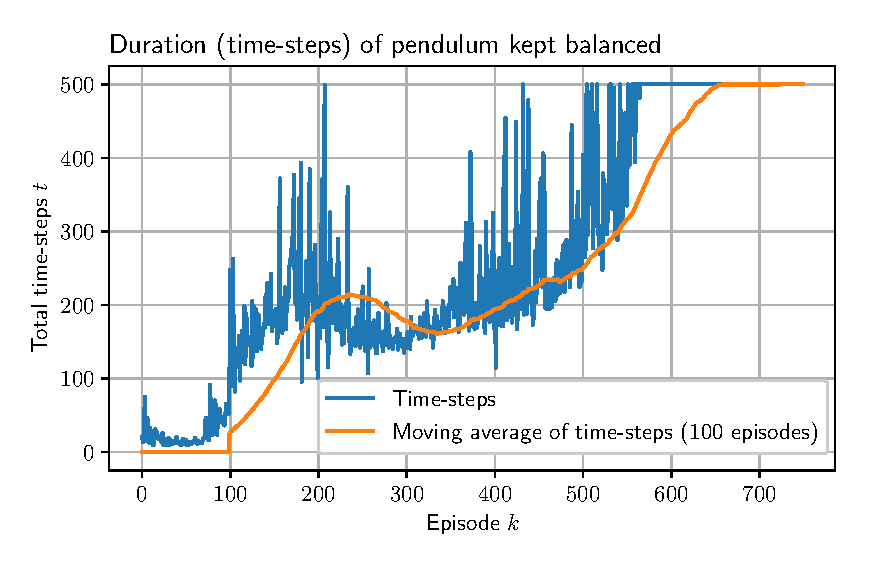
\includegraphics[width=1.0\textwidth]{PendulumDuration}
  % Matptlotlib Customized Settings
  % figsize=(6.25, 3.5)
  % loc='left', fontsize='large'
  \vspace{-1.5em}
  \caption{Duration of pendulum kept upright over training episodes.}
  \label{fig:PendulumDuration}
\end{figure}
% \begin{figure}[H]
%   \centering
%   \vspace{-1.0em}
%   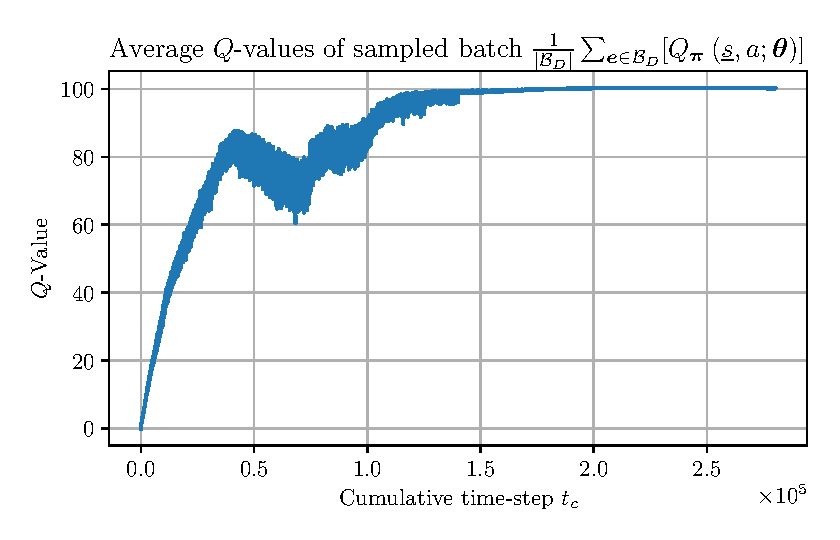
\includegraphics[width=1.0\textwidth]{QValuesPendulum}
%   % Matptlotlib Customized Settings
%   % figsize=(5.5, 3.5)
%   % ax.ticklabel_format(style='sci', axis='x', scilimits=(0,0))
%   % loc='left', fontsize='large
%   \vspace{-1.5em}
%   \caption{Progression of $Q$-values over the course of training.}
%   \label{fig:QValuesProgression}
% \end{figure}

\subsection{Patient-Specific Feature and Model Selection via Deep $Q$-Learning}
Inspired by the application of RL in controlling mechanical systems (i.e. balancing an inversed pendulum), the DQL algorithm is applied in this work to select an optimal feature subset of the extracted gait features, coupled along with a corresponding prediction (supervised learning) model to automatically assess gait poststroke. Earlier works by \cite{lee2020,lee2021} have applied DQL to develop a CDSS that automatically assesses a patient's ability in performing functional exercises, while delivering patient-specific relevant features for each corresponding task. In contrast, the method developed here is $(i)$ applied to the context of gait-assessment poststroke and $(ii)$ extended to include model selection. Model selection in this work will cover both the selection of a \emph{learning algorithm} and the subsequent \emph{hyperparameter tuning}. The issue of model selection is often described as more an art than a strict science \cite{raschka2020}, a notion underpinned by the ``No Free Lunch'' theorem by \cite{nofreelunch}, which proves that no single optimization algorithm can outperform all others across all possible problem spaces or datasets. Consequently, the selection of a model should be guided by the characteristics of the dataset, instead of a reliance on a universal ``best'' model. The learning algorithm and its corresponding optimal hyperparameters will be referred to as the \emph{prediction model} (PM) in the remainder of this paper.

\subsubsection{Contextualizing the Agent and Environment}
The environment is formulated as an episodic partially observable Markov Decision Process (POMDP), where an agent gradually learns by autonomously exploring different combinations of feature subsets and PMs to assess a patient's gait poststroke based on the extracted gait features. At each $k$-th episode, a randomly selected measured stride-pair yields a $D$-dimensional \emph{sample} $\sample_{k}$, comprised of the extracted gait features, alongside the corresponding medical-board's gait assessment $y_k$. The \emph{feature values} $x_{k,d}$ of the feature ${\feature}_{d} \in \fset$ make up the elements of $\sample_{k}$. The environment for a given time-step $t$ of the episode $k$, is represented by the state as formulated in (\ref{eq:ltfmstate})
\begin{equation}
    \begin{split}
        \nvec{s}_{t} &= \begin{bmatrix} {\nvec{\mathtt{X}}_t}^T & {\nvec{\mathtt{F}}_t}^T & g_t \end{bmatrix}^T \\
                     &= \begin{bmatrix} \mathtt{X}_{1,t} & \mathtt{X}_{2,t} & \cdots & \mathtt{X}_{D,t} & \mathtt{F}_{1,t} & \mathtt{F}_{2,t} & \cdots & \mathtt{F}_{D,t} & \mathtt{G}_{t} \end{bmatrix}^T \,.
    \end{split}
    \label{eq:ltfmstate}
\end{equation}
The episodic index will be dropped here for purposes of brevity. The vectors $\nvec{\mathtt{X}}_t$ and $\nvec{\mathtt{F}}_t$ denote the \emph{observed values} and \emph{observed features}, respectively. The \emph{selected PM} is denoted by $\mathtt{G}_{t}$. The agent is allowed to perform actions $a \in \mathcal{A}$, where the set $\mathcal{A}$ comprises three types of actions as shown in (\ref{eq:ltfmactions})
\begin{equation}
    \mathcal{A} = \begin{Bmatrix}
      \overbrace{a_0}^{\text{make prediction}} &
      \underbrace{\begin{matrix} a_1 & a_2 & \cdots & a_D \end{matrix}}_{\text{recruit feature}} &
      \underbrace{\begin{matrix} a_{D+1} & a_{D+2} & \cdots & a_{D+|\mathcal{G}|} \end{matrix}}_{\text{select PM}}
      \end{Bmatrix} \,.
    \label{eq:ltfmactions}
\end{equation}
The action $a_0$ fits the chosen PM $g$ to the training dataset, was has been trimmed to only include the selected subset of features $\fsubset$. The fitted PM is then used to predict $\hat{y}_k$, followed by computing the absolute error between the predicted and medical-board's gait assessment $\left| \hat{y}_k - y_k \right|$, which will be used to formulate the reward function. Actions $\left\{ a_{d} \,|\, 1 \leq d \leq D \right\}$ recruit feature ${\feature}_d$ to the subset of selected features $\fsubset$, whereas actions $\left\{ a_{j} \,|\, D+1 \leq j \leq D+|\mathcal{G}| \right\}$ chooses a PM $g_{j-D} \in \pmset$. The set ${\pmset} = \begin{Bmatrix} g_1 & g_2 & \cdots & g_{|\mathcal{G}|}\end{Bmatrix}$ denote the set of possible PMs from which the agent can choose from. The dynamics of the POMDP evolve deterministically according to (\ref{eq:ltfmdynamics}).
\begin{align}
    P(\nvec{s}, a) &=
    \begin{cases}
        \mathtt{X}_{d} = x_{d} \text{ and } \mathtt{F}_{d} = 1 & \text{if } a = a_{d} \text{, where } 1 \leq d \leq D \\
        \mathtt{G} = g_{j-D} & \text{if } a = a_{j} \text{, where } D+1 \leq j \leq D+|\mathcal{G}| \\
        T_{\text{end}} & \text{if } a = a_0 \\
    \end{cases}
    \label{eq:ltfmdynamics}
\end{align}
The episode begins with no features recruited and the initial state $\nvec{s}_0$ as shown in (\ref{eq:ltfminitialstate}).
\begin{equation}
    \begin{split}
        \nvec{s}_0 &= \begin{bmatrix} {\nvec{\mathtt{X}}_0}^T & {\nvec{\mathtt{F}}_0}^T & \mathtt{G}_{0} \end{bmatrix}^T \\
                     &= \begin{bmatrix} \mathtt{X}_{1,0} & \mathtt{X}_{2,0} & \cdots & \mathtt{X}_{D,0} & \mathtt{F}_{1,0} & \mathtt{F}_{2,0} & \cdots & \mathtt{F}_{D,0} & \mathtt{G}_{0} \end{bmatrix}^T \\
                     &= \begin{bmatrix} \bar{x}_{1} & \bar{x}_{2} & \cdots & \bar{x}_{D} & 0 & 0 & \cdots & 0 & \mathtt{G}_{0} \end{bmatrix}^T \,,
    \end{split}
    \label{eq:ltfminitialstate}
\end{equation}
where $\bar{x}_d$ denotes the average feature value of the feature ${\feature}_d$ computed from the training dataset. The observed feature $\mathtt{F}_d$ assumes the value $0$ to indicate feature's ${\feature}_d$ exclusion from the set of selected features $\fsubset$, and the PM $\mathtt{G}_{0}$ is initialized with a randomly chosen prediction model $g$ from the set $\mathcal{G}$. Consider a POMDP comprised of three features and two options of PMs as an example. At the current time-step $t={\xi}$, the recruited features include $\fsubset = \left\{ {\feature}_{1} \,, {\feature}_{3} \right\}$, and the PM $\mathtt{G}_{\xi} = g_1$ chosen. This would consequently yield the state $\nvec{s}_{\xi}$
\begin{equation}
    \begin{split}
        \nvec{s}_{\xi} &= \begin{bmatrix} \mathtt{X}_{1,\xi} & \mathtt{X}_{2,\xi} & \mathtt{X}_{3,\xi} & \mathtt{F}_{1,\xi} & \mathtt{F}_{2,\xi} & \mathtt{F}_{3,\xi} & \mathtt{G}_{\xi} \end{bmatrix}^T \\
                     &= \begin{bmatrix} x_{1} & \bar{x}_{2} & x_{3} & 1 & 0 & 1 & g_1 \end{bmatrix}^T \,.
    \end{split}
    \label{eq:ltfmexamplestate}
\end{equation}
The reward function is as given in (\ref{eq:ltfmreward}).
\begin{align}
    R(\nvec{s}, a) &=
    \begin{cases}
        -\lambda c \left( {\feature}_{d} \right) & \text{if } a = a_{d} \text{, where } 1 \leq d \leq D \\
        -c_{\fsubset} & \text{if } a = a_{d} \in \fsubset \text{, where } 1 \leq d \leq D \\
        -\lambda_{g} c_{g} \left( g_{j-D} \right) & \text{if } a = a_{j} \text{, where } D+1 \leq j \leq D+|\mathcal{G}| \\
        0 & \text{if } a = a_0 \text{, with } \left| \hat{y}_k - y_k \right| < \Delta \\
        -\left| \hat{y}_k - y_k \right| & \text{if } a = a_0 \text{, with } \left| \hat{y}_k - y_k \right| \geq \Delta \\
        -c_{g, \emptyset} & \text{if } a = a_0 \text{, with } \fsubset = \emptyset
    \end{cases}
    \label{eq:ltfmreward}
\end{align}
The penalties of recruiting a feature ${\feature}_d$ and choosing a PM $g_{j-D}$ are denoted by $c \left( {\feature}_{d} \right)$ and $c_{g} \left( g_{j-D} \right)$, respectively. They are multiplied by their respective factors $\lambda$ and $\lambda_{g}$. The agent is penalized by $c_{\fsubset}$ if it decides to select a feature ${\feature}_d$ which has already been previously recruited into $\fsubset$. When the agent decides to make a prediction, it is penalized by $\left| \hat{y}_k - y_k \right|$ if the absolute error is larger or equal a user-determined error tolerance $\Delta$. Otherwise, the agent is not penalized. However, if the agent decides to make a prediction without recruiting any features, a penalty of $c_{g, \emptyset}$ is incurred. The chosen PM is then fitted with the entire training dataset $\left( \dataset, \labels \right)$, which is in turn used to perform an inference on a ``background'' example, comprised of average feature values $\bar{\nvec{\mathtt{X}}} = \left[ \bar{x}_{1} \ \bar{x}_{2} \ \cdots \ \bar{x}_{D}\right]$ and deliver a prediction $\hat{y}_k$.

\subsubsection{Reconstruction of Gait Assessment}
The dataset used for modeling consists of 100 hemiparetic stroke patients which received a clinical examination and a full-body instrumented gait analysis. An interdisciplinary board of medical experts assigned each patient a Stroke Mobility Score (SMS) \cite{raab2020}, a multiple-cue clinical observational score comprised of six sub-scores each pertaining to a functional criterion of gait. The medical-board's gait-assessments (see Figure \ref{fig:LTFMvsBoard} were computed at subscore level as the mode of all individual recommendations. If the mode could not be defined, the subscore not in contention for the highest count was used as a tiebreaker. From the measurements, 904 measured stride pairs of 100 patients were obtained, 680 gait features extracted, and the dataset split 70/30 for training and testing. As a preprocessing step, expert knowledge was used to trim the features accordingly, followed by filtering out statistically non-discriminatory features. Detailed descriptions of these steps can be found in \cite{liaw2025}.

For each SMS subscore, the agent was trained on a batch size $|\mathcal{B}_{D}|=256$, sampled from the replay memory that stores the last $N=10000$ experiences, over 1500 episodes. The reward function was formulated with the penalties $c \left( {\feature}_d \right) = c_{g} \left( g_{j-D} \right) = 0.01$ and their respective factors $\lambda = \lambda_{g} = 1.0$, $c_{\fsubset} = 1.0$, $c_{g, \emptyset} = 5.0$, and $\Delta = 0.5$. The set $\mathcal{G}$ included random forest (RF), support vector machine (SVM), and multilayer perceptron (MLP) regression models. The RF and SVM regression models were implemented using scikit-learn \cite{scikit}, while the MLP regression model was similarly implemented using PyTorch \cite{pytorch}.

The optimal hyperparameters of each PM are selected by evaluating each hyperparameter combination (grid search) with a 3-fold cross-validation to select the hyperparameters that maximize the cross-validation estimate of the $R^2$. The SVM was implemented with a radial basis function as the kernel and grid-searched across the regularization parameter $C=\left\{ 0.1 \,, 0.5 \,, 1.0\right\}$, and the RF with 100 estimators and grid-searched across the maximum depth of trees $\left\{ 3 \,, 4 \,, 5 \right\}$. The MLP was implemented with four hidden layers with the number of units $\left\{ 32 \,, 32 \,, 16 \,, 8 \right\}$, trained with a batch size of 128 across 300 training epochs, AdamW learning rate of \num{1e-4}, and grid-searched across the weight decay $\lambda = \left\{ 0.01 \,, 0.1 \right\}$ and dropout probability $\left\{ 0.01 \,, 0.05 \right\}$.

The remaining hyperparameters not mentioned are left in their default values as implemented in scikit-learn and PyTorch. The policy and target networks were implemented as MLPs with two hidden layers, each with 1024 neurons, with the discount rate $\gamma = 0.99$ and soft update rate learning rate $\tau = $ \num{5e-4}. The parameters of the $Q$-network are optimized using an AdamW optimizer with the rate $l_r = $ \num{1e-5}. For the $\epsilon$-greedy algorithm, the agent selects a random action with the probability $\epsilon = \left( 0.9 - 0.05 \right) e^{-\frac{t_c}{1000}} + 0.05$. The algorithm was implemented using PyTorch \cite{pytorch}, alongside other standard Python packages such as NumPy \cite{numpy} and pandas \cite{pandas}. The training was performed on a computing system equipped with a 3.6 GHz AMD Ryzen\texttrademark{} 7 3700X CPU and an NVIDIA\textsuperscript{\textregistered{}} GeForce\textsuperscript{\textregistered{}} GTX 1650 GPU.

\section{Results}
The agent was trained on the training dataset and evaluated on the test dataset at patient-level. The performance of the resulting predictions for the SMS subscores and their summed SMS on the test dataset in terms of the $R^2$ are as shown in Table \ref{tab:ltfmresults}. This performance is comparable to the agreement of each expert recommendation with the collective decisions of the medical-board (see Figure \ref{fig:LTFMvsBoard}). For each evaluation of the test data, the agent was able to optimally select a feature set and a PM for a given stride-pair, yielding excellent predictive performance and delivering patient-specific key features, which could help medical experts identify personalized key therapeutic targets.
\begin{table}[H]
  \caption{Performance of RL agents on the test dataset in terms of $R^2$, and corresponding ICC\textsubscript{1.1} of the medical-board assessments.}
  \label{tab:ltfmresults}
  \begin{tabular}{|l|l|l|l|}
    \hline
    \textbf{SMS} & \textbf{Feature subset} & \textbf{$R^2$} & \textbf{ICC\textsubscript{1.1}} \\
    \textbf{subscore} & $|\fsubset|$ & & \\
    \hline
    Trunk-SMS     & 241 of 680 features & 0.59 $\,$ & 0.65 \\
    Leg-SMS       & 188 of 356 pre-selected features & 0.56 $\,$ & 0.73 \\
    Arm-SMS       & 99 of 330 pre-selected features & 0.54 $\,$ & 0.72 \\
    Speed-SMS     & 31 of 32 pre-selected features & 0.78 $\,$  & 0.72 \\
    Fluency-SMS   & 263 of 680 features & 0.73 $\,$ & 0.72 \\
    Stability-SMS & 238 of 680 features & 0.82 $\,$ & 0.83 \\
    \hline
    \multicolumn{2}{|l|}{Combination of subscore models to predict the SMS} & 0.83 & 0.88 \\
    \hline
  \end{tabular}
\end{table}
\begin{figure}[!h]
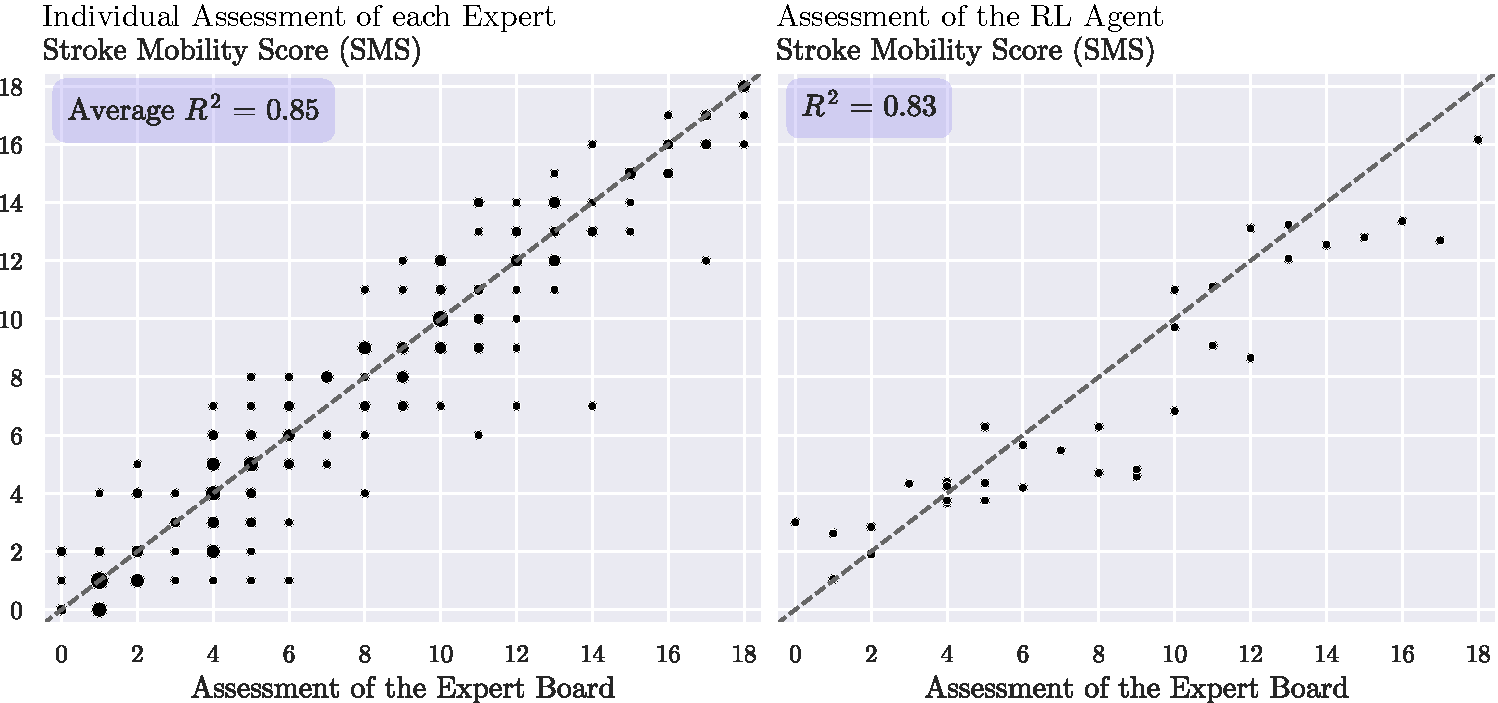
\includegraphics[width=\textwidth]{DoctorsvsBoard_TestSplit_and_LTFMJRMCC.pdf}
\caption{Scatterplots showing how the individual experts (left) and RL agent (right) compare with the medical-board's gait assessment (abscissa) in terms of the SMS.} \label{fig:LTFMvsBoard}
\end{figure}
To obtain a general overview of the salient features for the varying degrees of gait impairment, inference is performed on the training dataset, and the frequency of recruited features summed per SMS subscore. The intuititon here is that patients assigned the same SMS subscore should exhibit similar underlying physical characteristics, represented by a subset of key features. Upon observing a patient, a well-trained agent then recruits the features that make up the underlying pattern learned from patients of similar physical status. Consequently, the recruitment frequency of a feature can serve as an indication of the feature's representativeness with respect to a given SMS subscore group. Taking Fluency-SMS as an example, the top seven features and progression of the averaged $Q$-values per sampled batch during training are as shown in Table \ref{tab:featuresRecruitmentFrequency} and Figure \ref{fig:QValuesProgression}, respectively.
\begin{table}[H]
  \caption{Top features by recruitment count for predicting SMS-Fluency. NAV denotes the normalized angular velocity, as described in \cite{liaw2025}.}
  \label{tab:featuresRecruitmentFrequency}
  \begin{tabular}{|p{0.075\textwidth}|p{0.23\textwidth}|p{0.23\textwidth}|p{0.23\textwidth}|p{0.23\textwidth}|}
    \hline
    \multirow{2}{*}{\textbf{Rank}} & \multicolumn{4}{c|}{\textbf{SMS-Fluency}} \\ \cline{2-5}
       & \textbf{Score 0} & \textbf{Score 1} & \textbf{Score 2}  & \textbf{Score 3} \\ \hline
    1  & Thorax Rotation  & Shoulder Flex./Ex. & Pelvis Tilt   & Pelvis Tilt   \\
       & Angle contra.    & NAV ipsi.          & NAV ipsi.     & NAV ipsi.     \\
       & (Swing min.)     & (Stride median)    & (Stride min.) & (Stride min.) \\ \hline
    2  & Ankle Dorsiflexion & Spine Rotation   & Shoulder Flex./Ex. & Shoulder Flex./Ex. \\
       & Angle contra       & NAV ipsi.        & NAV ipsi.          & NAV ipsi.          \\
       & (Stance max.)      & (Stride max.)    & (Stride median)    & (Stride median)    \\ \hline
    3  & Shoulder Flex./Ex. & Ankle Dorsiflexion & Ankle Dorsiflexion & Ankle Dorsiflexion \\
       & NAV ipsi.          & Angle contra.      & Angle contra.      & Angle contra.      \\
       & (Stride median)    & (Stance max.)      & (Stance max.)      & (Stance max.)      \\ \hline
    4  & Pelvis Tilt   & Spine Side Tilt & Spine Side Tilt & Spine Side Tilt \\
       & NAV ipsi.     & Angle contra.   & Angle contra.   & Angle contra.   \\
       & (Stride min.) & (Stance max.)   & (Stance max.)   & (Stance max.)   \\ \hline
    5  & Spine Side Tilt & Pelvis Rotation & Pelvis Tilt   & Pelvis Tilt   \\
       & Angle contra.   & Angle contra.   & NAV contra.   & NAV contra.   \\
       & (Stance max.)   & (Stride min.)   & (Stance max.) & (Stance max.) \\ \hline
    6  & Thorax Tilt   & Pelvis Tilt   & Elbow Flex./Ex. & Elbow Flex./Ex. \\
       & NAV ipsi.     & NAV ipsi.     & Angle ipsi.     & Angle ipsi.     \\
       & (Stride max.) & (Stride min.) & (Stride median) & (Stride median) \\ \hline
    7  & Pelvis Tilt   & Ankle Dorsiflexion & Spine Rotation & Spine Rotation \\
       & NAV contra.   & Angle contra.      & NAV ipsi.      & NAV ipsi.      \\
       & (Stance max.) & (Stride max.)      & (Stride max.)  & (Stride max.)  \\ \hline
    \end{tabular}
\end{table}
\begin{figure}[!h]
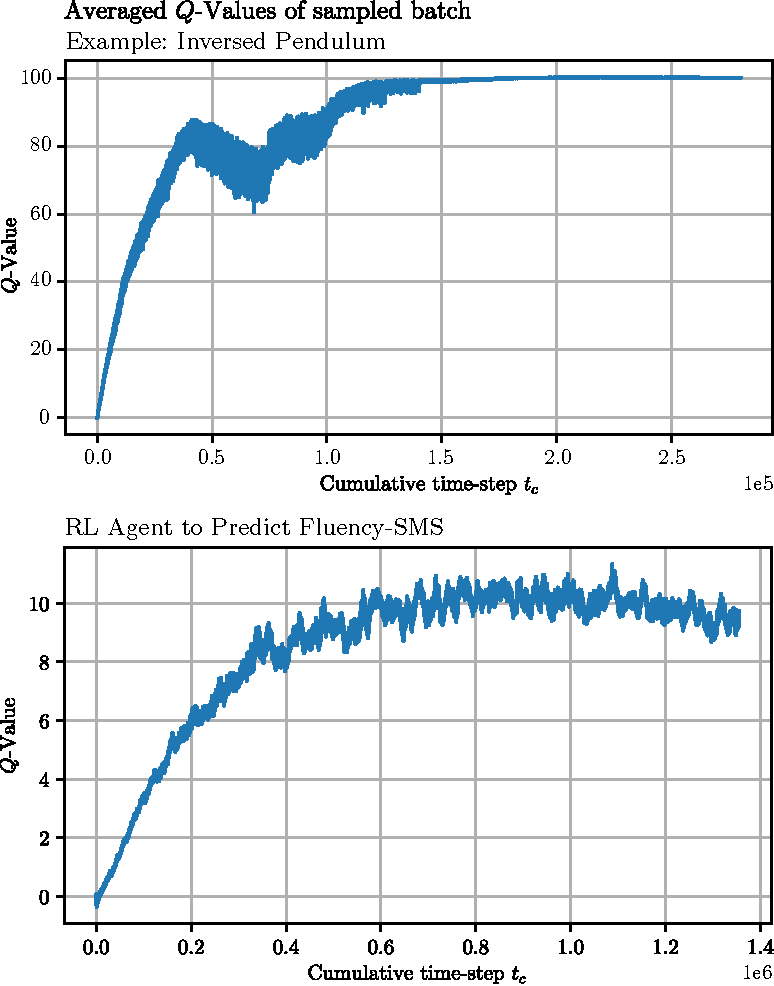
\includegraphics[width=0.75\textwidth]{QValuesFluency_and_Pendulum.pdf}
\caption{Averaged $Q$-Values per sampled batch at each training iteration for the example of balancing an inversed pendulum (top) and predicting the Fluency-SMS (bottom).} \label{fig:QValuesProgression}
\end{figure}

% %% Stride-Pair 1::
% %% Stride-Pair 2::
% Consider the following two stride-pairs, which will be referred to as SPI and SPII from the test dataset. SPI is a measured stride-pair of a critically affected patient (SMS of XX), and SPII, that of a mildly affected patient (SMS of XX). Both these handpicked examples have correctly predicted SMS, but not all predicted SMS subscores are necessarily correct. The true SMS subscores are displayed in brackets, next to the predicted subscores in Table \ref{tab:handpickedLTFMExamples} and as one can see, the selected key features vary depending on the physical status of a patient. The features listed in Table \ref{tab:handpickedLTFMExamples} are sorted in accordance to its relevance in terms of distinguishing samples of the selected stride-pair's assigned subscore from the remaining three subscores, quantified by the mutual information (cite??).

% \begin{table}[H]
%   \centering
%   \begin{tabular}{@{}l@{\hspace{0.25em}}|p{0.4\textwidth}p{0.4\textwidth}}
%     \hline
%     \textbf{Sub-} & \textbf{<Example A>} & \textbf{<Example B>} \\
%     \textbf{score} & $\quad$ \textbf{SMS: XX (critical)} & $\quad$ \textbf{SMS: XX (mild)} \\
%     \hline
%     \multirow{5}{*}{$\hspace{0.95em}$\makebox[0.75em]{\rotatebox{90}{\textbf{Trunk-SMS }}}}
%     & \textbf{Predicted score: XX} (XX) & \textbf{Predicted score: XX} (XX) \\ \cline{2-3}
%     & Feature A.2 & Feature B.2 \\
%     & Feature A.3 & Feature B.3 \\
%     & Feature A.4 & Feature B.4 \\
%     & $\cdots$ (XX features in total) & $\cdots$ (XX features in total) \\ \hline
%     \multirow{5}{*}{$\hspace{0.95em}$\makebox[0.75em]{\rotatebox{90}{\textbf{Leg-SMS }}}}
%     & \textbf{Predicted score: XX} (XX) & \textbf{Predicted score: XX} (XX) \\ \cline{2-3}
%     & Feature A.2 & Feature B.2 \\
%     & Feature A.3 & Feature B.3 \\
%     & Feature A.4 & Feature B.4 \\
%     & $\cdots$ (XX features in total) & $\cdots$ (XX features in total) \\ \hline
%     \multirow{5}{*}{$\hspace{0.95em}$\makebox[0.75em]{\rotatebox{90}{\textbf{Arm-SMS }}}}
%     & \textbf{Predicted score: XX} (XX) & \textbf{Predicted score: XX} (XX) \\ \cline{2-3}
%     & Feature A.2 & Feature B.2 \\
%     & Feature A.3 & Feature B.3 \\
%     & Feature A.4 & Feature B.4 \\
%     & $\cdots$ (XX features in total) & $\cdots$ (XX features in total) \\ \hline
%     \multirow{5}{*}{$\hspace{0.95em}$\makebox[0.75em]{\rotatebox{90}{\textbf{Speed-SMS }}}}
%     & \textbf{Predicted score: XX} (XX) & \textbf{Predicted score: XX} (XX) \\ \cline{2-3}
%     & Feature A.2 & Feature B.2 \\
%     & Feature A.3 & Feature B.3 \\
%     & Feature A.4 & Feature B.4 \\
%     & $\cdots$ (XX features in total) & $\cdots$ (XX features in total) \\ \hline
%     \multirow{5}{*}{$\hspace{0.95em}$\makebox[0.75em]{\rotatebox{90}{\textbf{Fluency-SMS }}}}
%     & \textbf{Predicted score: XX} (XX) & \textbf{Predicted score: XX} (XX) \\ \cline{2-3}
%     & Feature A.2 & Feature B.2 \\
%     & Feature A.3 & Feature B.3 \\
%     & Feature A.4 & Feature B.4 \\
%     & $\cdots$ (XX features in total) (XX) & $\cdots$ (XX features in total) (XX) \\ \hline
%     \multirow{5}{*}{$\hspace{0.95em}$\makebox[0.75em]{\rotatebox{90}{\textbf{Stability-SMS }}}}
%     & \textbf{Predicted score: XX} & \textbf{Predicted score: XX} \\ \cline{2-3}
%     & Feature A.2 & Feature B.2 \\
%     & Feature A.3 & Feature B.3 \\
%     & Feature A.4 & Feature B.4 \\
%     & $\cdots$ (XX features in total) & $\cdots$ (XX features in total) \\ \hline
%   \end{tabular}
%   \caption{Two examples from the test dataset, each with their respective subset of features recruited by the agent to predict each SMS subscores}
%   \label{tab:handpickedLTFMExamples}
% \end{table}

\section{Discussion}
The SMS and the Stability-SMS models perform very well ($R^2$ $> 0.8$), while the other models perform well ($R^2$ $> 0.5$). Unsurprisingly, the performances correlate strongly [Cohen \cite{cohen1988}, $p=0.08$, $r=0.71$] with the corresponding interrater reliabilities ICC\textsubscript{1.1} of the medical-board. Though the individual subscore models do not perform perfectly well, they compensate for one another when formulating the SMS. There are nonetheless, a few shortcomings and issues that should be addressed. The first is the number of features recruited by the agent to make a prediction. While penalizing the agent everytime it recruits a feature has helped produce a reduced feature subset, one can nonetheless see in Table \ref{tab:featuresRecruitedReduction} that the number of recruited features is still considerably high.
\begin{table}[H]
  \caption{Number of original features, average number of features recruited by the agent (rounded to closest integer), and the reduction in percentage.}
  \label{tab:featuresRecruitedReduction}
  \begin{tabular}{|l|l|l|l|}
    \hline
    \textbf{SMS} & \multicolumn{3}{c|}{\textbf{Number of features}} \\ \cline{2-4}
    \textbf{Subscore}  & \textbf{Original} $|\fset|$ & \textbf{Average} $|\fsubset|$ & \textbf{Reduction} $[\%]$ \\ \hline
    Trunk-SMS     & 241 & 140 & 41.9 \\ 
    Leg-SMS       & 188 & 113 & 39.9 \\ 
    Arm-SMS       & 99  & 59  & 40.4 \\
    Speed-SMS     & 31  & 21  & 32.2 \\
    Fluency-SMS   & 253 & 141 & 44.3 \\
    Stability-SMS & 238 & 133 & 44.1 \\ \hline \hline
    \multicolumn{3}{|c|}{\textbf{Average reduction of number of features}} & 40.5 \\ \hline
  \end{tabular}
\end{table}
This could be counterintuitive and pose the risk of overwhelming clinicians with information \cite{lee2020,lee2021}. It would thus be beneficial to reduce the number of recruited features to an amount, that lies within established cognitive processing limits (e.g. $7 \pm 2$) \cite{miller1994}. While this might exclude a few key features, interpretability is often prioritized over predictive accuracy in developing CDSSs, as they should serve as an aid rather than a replacement for human experts. Secondly, the agent was also observed to alternate between PM numerous times within an episode before finally deciding to make a prediction. This seems to reflect ``undecisiveness'', akin to that of a human ML practitioner. Thirdly, medical diagnostic erros are often asymmetrical. While an overpessimistic result (a false positive) may lead to unnecessary follow-up testing or temporary patient anxiety, the consequences of overoptimistic results (a false negative) can result in the catastrophic delay of life-saving treatment, or doctors recommending futile, aggressive care instead of more beneficial palliative care \cite{christakis2000}.

A key highlight of this RL-based approach is the versatility it offers by reformulating the reward function to account for these issues. For instance, to encourage the agent to limit the number of recruited features to around seven, the penalty of recruiting a feature can be progressively increased after the number of recruited features $|\fsubset|$ exceeds a user-defined threshold. If there exists a feature that possesses an undesired characteristic such as being difficult to interpret or challenging to obtain, one could also set a higher penalty for that feature. Similarly, one could also penalize the agent more for choosing a MLP, over less computationally taxing ones like SVM. To steer the agent away from making overoptimistic diagnostic errors, errors where the predicted medical score is lower than that of the true score can be weighed more heavily. Shown in (\ref{eq:HypotheticalRewardFunction}) is a hypothetical reward function, that could account for the aformentioned issues.
\begin{align}
    R(\nvec{s}, a) &=
    \begin{cases}
      -\lambda_{d} c \left( {\feature}_{d} \right) & \text{if } a = a_{d} \text{, where } 1 \leq d \leq D , \,\, \lambda_{d} \in \nvec{\lambda}_{\fset}\\
      -\lambda c^{*}(|\fsubset|) & \text{if } a = a_{d} \text{ and } |\fsubset| > |{\fsubset}^{*}| \text{, where } 1 \leq d \leq D \\
      -c_{\fsubset} & \text{if } a = a_{d} \in \fsubset \text{, where } 1 \leq d \leq D \\
      -\lambda_{j} c_{g} \left( g_{j-D} \right) & \text{if } a = a_{j} \text{, where } D+1 \leq j \leq D+|\mathcal{G}| , \,\, \lambda_{g} \in \nvec{\lambda}_{\pmset}\\
      0 & \text{if } a = a_0 \text{, with } \left| \hat{y}_k - y_k \right| < \Delta \\
      -\left| \hat{y}_k - y_k \right| & \text{if } a = a_0 \text{, with } \left| \hat{y}_k - y_k \right| \geq \Delta \text{ and } \hat{y}_k > y_k \\
      -\lambda_{y} \left| \hat{y}_k - y_k \right| & \text{if } a = a_0 \text{, with } \left| \hat{y}_k - y_k \right| \geq \Delta \text{ and } \hat{y}_k < y_k\\
      -c_{g, \emptyset} & \text{if } a = a_0 \text{, with } \fsubset = \emptyset
    \end{cases}
    \label{eq:HypotheticalRewardFunction}
\end{align}
The penalty factors for recruiting a feature and PM can be stored in their respective lookup tables $\nvec{\lambda}_{\fset} = \left[ {\lambda}_{1} \ {\lambda}_{2} \ \cdots \ {\lambda}_{d} \ \cdots \ {\lambda}_{D}\right]$ and $\nvec{\lambda}_{\pmset} = \left[ {\lambda}_{1} \ {\lambda}_{2} \ \cdots \ {\lambda}_{j} \ \cdots \ {\lambda}_{|\pmset|}\right]$, where the each penalty $\lambda$ is user-defined. To steer the agent towards selecting a user-desired number of features $|{\fsubset}^{*}|$, the penalty of recruiting a feature can be progressively increased by $c^{*}(|\fsubset|)$, as a function of the number of recruited features $|\fsubset|$. In the case of a prediction error larger than the error tolerance $\Delta$, the penalty for predicted scores larger than that of the true score $\hat{y}_k > y_k$ is the absolute difference, whereas the penalty for predicted scores smaller than the true score $\hat{y}_k < y_k$ is the absolute difference multiplied by a user-defined factor $\lambda_y$.

One limitation that should be accounted for is the unbalanced datasets on which the agent is trained on. This could especially be problematic during training because a sample is randomly chosen at every iteration. This stochastic sampling might lead to an agent that is heavily biased toward the majority class, failing to generalize to rarer but potentially more critical scenarios. However, to account for this, each sample is weighted to account for two source of biases as described in \cite{liaw2025}. A second issue would be a technical one, namely the sheer scale of the required iterations. This attached computational cost is further multiplied when one factors in hyperparameter tuning. Therefore, to effectively explore the hyperparameter space and ensure model robustness, one should leverage cloud supercomputers, that enables massive parallelization to manage the vast search space.

One lesson learned from applying DQL in balancing an inversed pendulum, as described in the earlier section, is the importance of beginning with a reasonably ``good'' initial estimate for solution convergence. Given the simple implementation described earlier, the controller would very unlikely ever swing the pendulum into its upright position, if the pendulum was initially simply hanging from the revolute joint. Similarly here, the agent would very unlikely find a good subset of features, if it was presented with all 680 features. Moreover, if the original set of features were all included, the number of selected features by the agent would be tremendously overwhelming to effectively help a clinician.
% Run a round of ltfm with all 680 feature to prove the point.

\section{Conclusion}
In conclusion, the gait assessments in terms of the SMS, prescribed by an interdisciplinary medical board was well reproduced from gait data by training an agent that can dynamically select salient features, and a corresponding PM. More importantly, the agent was able to select a subset of features specific to a patient. These patient-specific features could potentially aid clinicians in better designing personalized therapy, especially with earlier research \cite{lee2020,pistacchi2017,huang2016,biase2020} indicating the importance of accounting for inter-patient variability, and the relevant biomarkers evolving as a function of disease progression. These synergistic interactions between system, and experts may improve the quality in diagnosis and help objectify therapeutic targets.


\bibliographystyle{splncs04}
\bibliography{references}

\end{document}
